% ===============================================================================
% = LaTeX Beamer Template des Arbeitsbereichs Sicherheit in verteilten Systemem
% = (c) 2016 Prof. Dr. Hannes Federrath, Uni Hamburg, Fachbereich Informatik
% = https://svs.informatik.uni-hamburg.de
% =
% = Weitgehend in Übereinstimmung mit dem Corporate Design 2016 der UHH:
% = https://www.uni-hamburg.de/beschaeftigtenportal/services/oeffentlichkeitsarbeit/corporate-design.html
% = 
% ===============================================================================
%
\documentclass[t,aspectratio=169]{beamer} 
% Option t              Place text of slides at the (vertical) top of the slides.
% Option handout        Ein PDF ohne Pausen und Overlayeffekte erzeugen.
% Option aspectratio=43 169 => 16:9, 1610 => 16:10, 43 => 4:3
\usepackage[utf8]{inputenc}
\usepackage[ngerman]{babel}
\usepackage{graphicx,xcolor}
\usepackage[T1]{fontenc} % 8-Bit-Zeichen; ermöglicht korrektes Kopieren von Umlauten aus dem pdf 
\bibliography{bib}
\bibliographystyle{ieee}
\usepackage{biblatex}
\addbibresource{bib.bib}

% SVS-Theme benutzen
\usetheme{svs2021}

% =============================
% = Ab hier Inhalte ändern... 
% =============================

\title{Security and Privacy Concerns in Federated Learning: An Introduction}
% \subtitle{Ein Vorschlag}
\author[]{Jonas Müller, Rebekka Schnoor}
% \institute[Uni Hamburg]{Universität Hamburg · Fachbereich Informatik}
\date{30.04.2026} % Ausblenden geht mit leerem Inhalt: \date{}
% \titlegraphic{\uhhlogo} % Logo für Titelseite, UHH-Logo ist Standard
\eventlocation{Master Project Seminar Data Protection and Data Security, Hamburg, 30. April 2026} % rechts oben auf Titelseite

\begin{document}

\begin{frame}
	% Die Titelseite erscheint nach erneutem Übersetzen korrekt.
	\maketitle
\end{frame}

\begin{frame}
	\frametitle{Agenda}
	% Die Gliederung erscheint nach erneutem Übersetzen korrekt.
	% Die Gliederung wird im Dokument fortlaufend durch \section{} und \subsection{} definiert. Die Folien selbst haben keinen Einfluss auf die Gliederung.
	\tableofcontents
	% Hinweis: Das pandoc-Template benutzt \tableofcontents[hideallsubsections] zur Erzeugung einer Gliederung. Daher werden in der Markdown-Version nur die Überschriften der ersten Ebene (#) im Inhaltsverzeichnis angezeigt. Die normalerweise bei Verwendung von pandoc erzeugten Zwischenfolien für jede Überschrift der ersten Ebene werden im Theme unterdrückt. 
\end{frame}

\section{Federated Learning} % erscheint in Agenda
\subsection{Motivation} % erscheint in Agenda
\subsection{Training Process}
\subsection{Limitations} % erscheint in Agenda

\begin{frame}{Federated Learning: Motivation}
    \begin{columns}
        \begin{column}{0.5\textwidth}
            \begin{itemize}
                \item Training one central model on distributed data
                \item Transmitting full datasets causes high communication cost
                \item Data may contain sensitive information (medical data, PII)
            \end{itemize}
            \begin{alertblock}{Solution}
                Train locally on datasets and only communicate updates
            \end{alertblock}
        \end{column}
        \begin{column}{0.3\textwidth}
        \begin{center}
            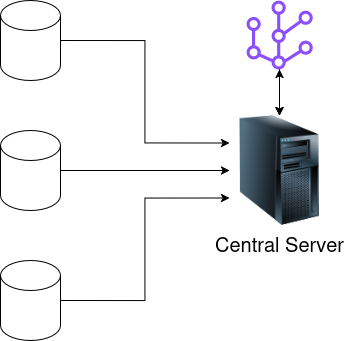
\includegraphics[width = \textwidth]{img/distributed_training.png}
        \end{center}
        \end{column}
    \end{columns}
\end{frame}

\begin{frame}
	\frametitle{Federated Learning: Initialization of local models}
    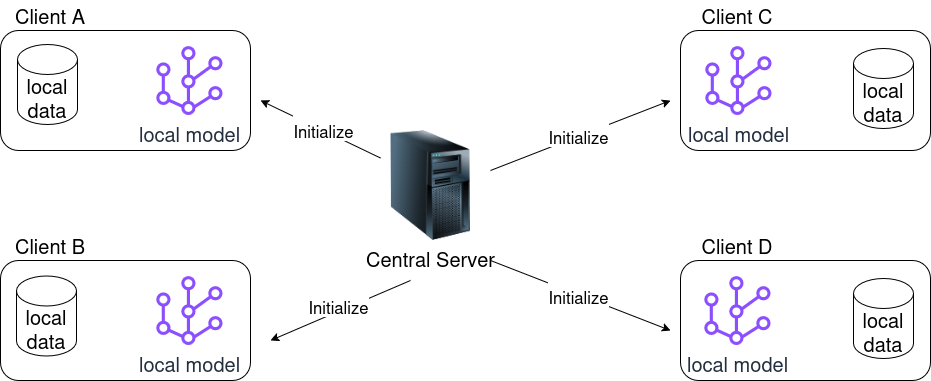
\includegraphics[width=\textwidth]{img/FL_init.png}
\end{frame}
\begin{frame}
	\frametitle{Federated Learning: Training}
    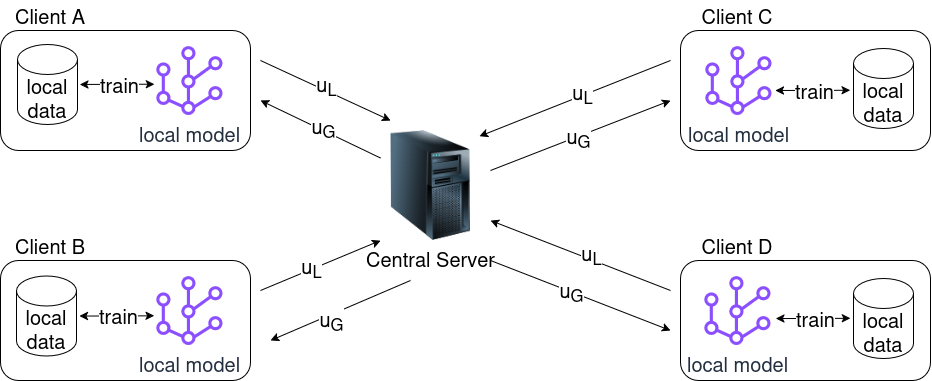
\includegraphics[width=\textwidth]{img/FL_train.png}
%TODO add legend
\centering
u$_L$ - local updates\\
u$_G$ - updated global model
\end{frame}

\begin{frame}{Federated Learning}
\begin{columns}
    \begin{column}{0.5\textwidth}
        \begin{enumerate}
            \item Initialize global model
            \item Distribute model to clients
            \item Clients perform local training
            \item Server aggregates updates
            \item Share updated model
        \end{enumerate}
        
     \vspace{0.2cm}   
    Repeat 2.-5. until convergence

    \end{column}
    \begin{column}{0.4\textwidth}
        \begin{center}
            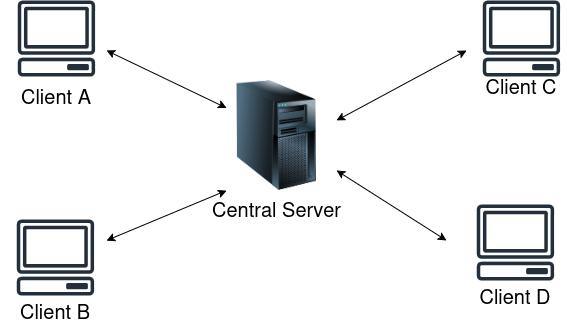
\includegraphics[width=\linewidth]{img/FL_train_simplified.png}
        \end{center}
        
    \end{column}
\end{columns}  
\vspace{0.2cm}
\begin{alertblock}{Main Limitation: Dependence on Server}
\begin{itemize}
    \item [] Requires trust in the central server
    \item [] Scalability bottleneck
\end{itemize}         
\end{alertblock}

\end{frame}


\section{Decentralized Federated Learning} % erscheint in Agenda
\begin{frame}{Decentralized Federated Learning}
    \begin{center}
        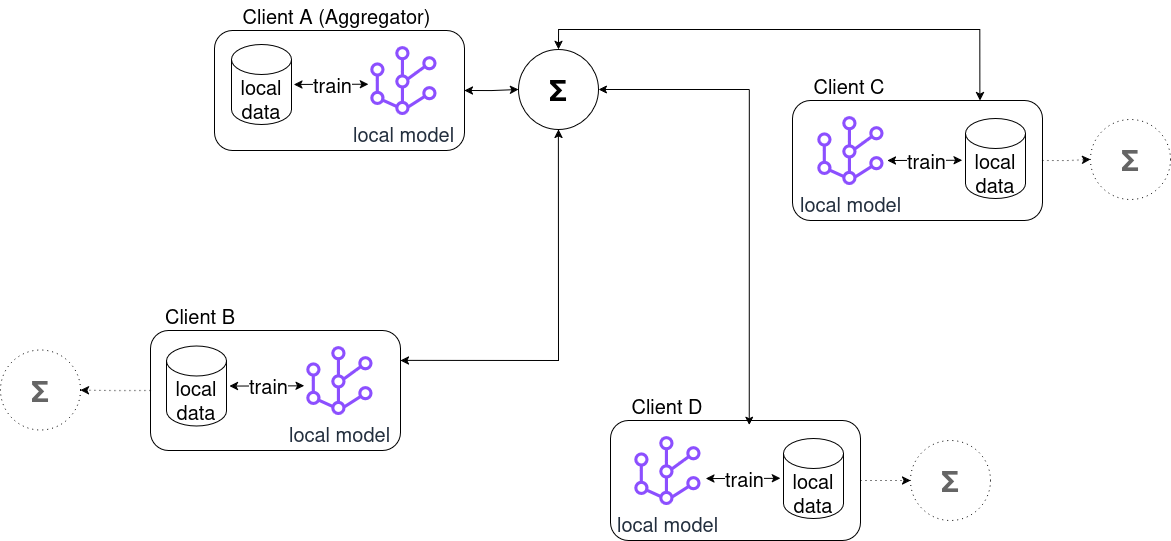
\includegraphics[width=0.95\textwidth]{img/DFL.png}
    \end{center}

\end{frame}

\begin{frame}{Decentralized Federated Learning}
\begin{columns}
    \begin{column}{0.5\textwidth}
        \begin{enumerate}
            \item Local training and model aggregation as in centralized FL
            \item Clients take turns acting as aggregators
            \item Model updates are exchanged via peer‑to‑peer communication
            \item Commonly uses blockchain to ensure traceability and immutability
        \end{enumerate}

        \begin{alertblock}{Main Risks}
        \begin{itemize}
            \item[] Blockchain-related vulnerabilities 
            \item[] Malicious clients
        \end{itemize}
        \end{alertblock}
    \end{column}
    \begin{column}{0.5\textwidth}
        \begin{center}
            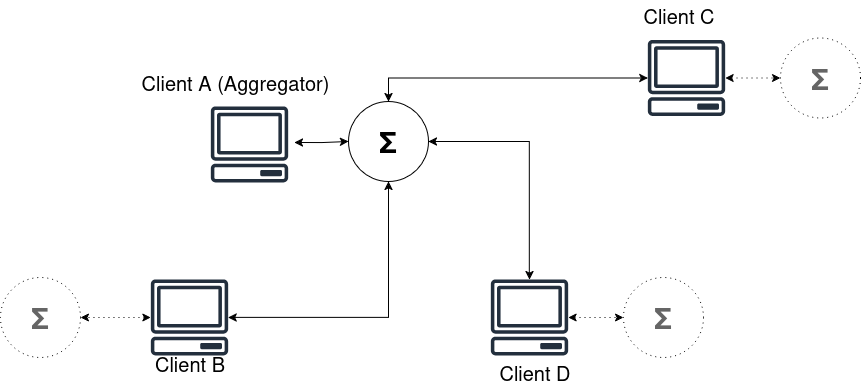
\includegraphics[width=\linewidth]{img/DFL_simplified.png}
        \end{center}
    \end{column}
\end{columns}  
\end{frame}

\subsection{Blockchain}
\begin{frame}{Blockchain}
\begin{columns}
\begin{column}{0.5\textwidth}
    \begin{figure}
    
\includegraphics[width=\textwidth]{img/blockchain.png}
    \caption{Structure of a blockchain}
    \label{blockchain}
\end{figure}
\end{column}
\begin{column}{0.5\textwidth}
    \begin{itemize}
        \item Tamper‑resistant, append‑only log storing model updates and aggregation steps
        \item Decentralized coordination using Smart contracts to enforce participation rules and aggregation conditions
    \end{itemize}
    \begin{alertblock}{Limitations}
        \begin{itemize}
            \item[] Latency and computational overhead
            \item[] Continuous storage growth
            \item[] Known vulnerabilities
        \end{itemize}
    \end{alertblock}
\end{column}
\end{columns}

\end{frame}

\begin{frame}{Blockchain-based DFL \cite{Hallaji_2024}}
    \begin{figure}
        %\centering
        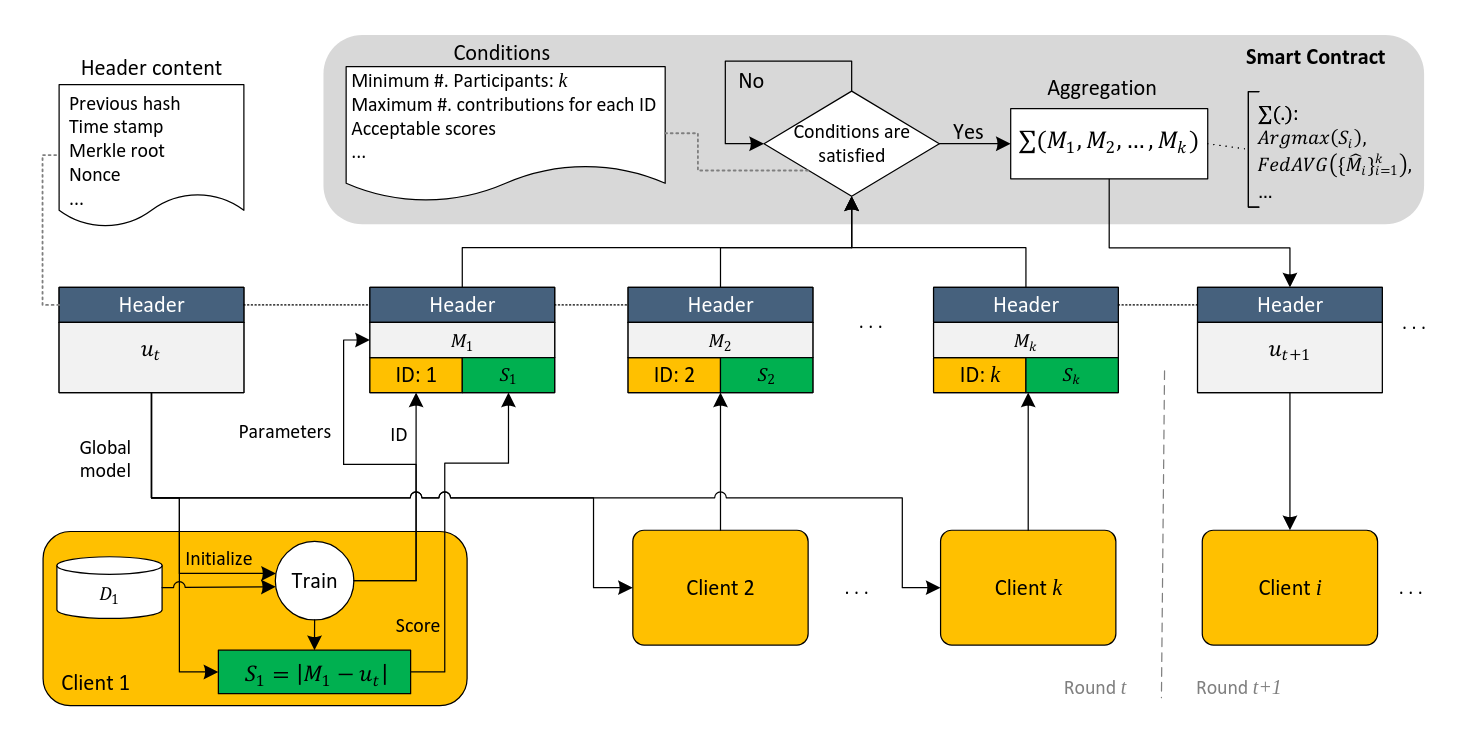
\includegraphics[width=0.95\linewidth]{img/bc_dfl.png}
        %\caption{Smart contracts validate contributions and trigger aggregation when conditions are met}
        \label{fig:blockchain_dfl}
    \end{figure}
\end{frame}
\section{Threats}
\subsection{Security}

\begin{frame}{Blockchain-specific Vulnerabilities}
\vspace*{\fill}
    \begin{itemize}
        \item Communication disruption (DDoS)
        \begin{itemize}
            \item []Fill up the blockchain buffer with spam data
        \end{itemize}
        \item  Consensus Attacks
        \begin{itemize}
            \item []Create multiple fake nodes to influence control consensus mechanism
        \end{itemize}
        \item Routing Attacks
                \begin{itemize}
            \item[] Manipulate package routing to change blockchain structure
        \end{itemize}
        \item Privacy poisoning
        \begin{itemize}
            \item[] Insert personal data into a blockchain block, causing non-compliance with legal requirements
        \end{itemize}
    \end{itemize}
\vspace*{\fill}
\end{frame}
\begin{frame}{Attacks on Model Performance}
    \vspace*{\fill}
    \begin{itemize}
        \item Data Poisoning
        \begin{itemize}
            \item[] Train local model on artificially created dataset to inject backdoors, then share poisoned gradients
        \end{itemize}
        \item Model Poisoning
        \begin{itemize}
            \item[] Maliciously influence global model training, e.g. by changing the objective function
        \end{itemize}
        \item (Evasion Attacks)
        \begin{itemize}
            \item[] Decrease model performance during inference by manipulating input data. Can be facilitated by poisoning attacks during training, but is not inherently tied to FL
        \end{itemize}
    \end{itemize}
    \vspace*{\fill}
\end{frame}
\subsection{Privacy}
\begin{frame}{Attacks on Privacy}
    \vspace*{\fill}
    \begin{itemize}
        \item Model Inversion
        \begin{itemize}
            \item[] Approximate client data using generative models, e.g. GANs
        \end{itemize}
        \item Inference Attacks: 
        \begin{itemize}
        \item[] Infer information about a dataset based on the model updates generated by a client using that dataset
        \begin{itemize}
            \item Feature Inference: Gain information about sensitive features
            \item Membership Inference: Determine if a data point was used to train the model
            \end{itemize}
        \end{itemize}
    \end{itemize}
    \vspace*{\fill}
\end{frame}

\begin{frame}{References}
\printbibliography
    
\end{frame}
\end{document}